\chapter{Introduction}

\section{Who was Kowalevski?}
\begin{wrapfigure}{i}{0.25\textwidth}
\centering
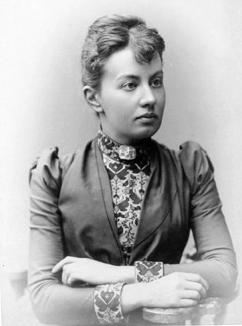
\includegraphics[width=0.25\textwidth]{kovalevskaya_8}
\end{wrapfigure}

Sofya Vasilyevna Kovalevskaya (1850-1891) was a Russian mathematician. For various reasons, including the theorem at the center of this discussion, she remains one of the most significant female figures in the history of this discipline.

First of all, it is important to emphasize that from now on we will refer to her by the name she used to sign her publications, namely Kowalevski.

To leave Russia, she had to enter into a sham marriage; she married a man with whom she had no real romantic relationship and from whom she often remained geographically distant. This allowed her to continue her studies in Germany, where she met Karl Weierstrass, one of the most influential mathematicians of his time. After an initial meeting in the professor's study, their relationship continued to develop thanks to Sofya's evident mathematical talents, which Weierstrass could not help but encourage. He continued to give her private lessons and eventually supervised her research work.

Regarding Kowalevski's political views, we can assert with historical certainty her closeness to feminist movements and socialist and radical ideas, which can be traced back to her family background and the insights she gained during her life experiences in the states of modern-day Europe. It is certainly noteworthy that she received various copies of radical magazines of that time from her sister Anna, discussing the so-called ancient nihilism\footnote{For the ancient nihilists, science, and not religion and superstition, appeared as the most effective means to help the population and therefore represented truth and progress.}.

What we want to focus on is not her political, social, and philosophical ideas but rather her contribution to mathematics. Kowalevski, with the help of what we can call her mentor, made several important discoveries. After several years of collaboration, she managed to publish three doctoral theses in a single year: 1874. This was not the only notable aspect; she was also the first woman to obtain a doctorate, made possible by Weierstrass's support, as evidenced by a letter he wrote to his colleague Fuchs at the University of Berlin regarding the approval of Sofya's theses. Furthermore, her publications, besides being significant for the reasons just mentioned, proved to be milestones in mathematics. In particular, the topics covered were:
\begin{itemize}
\item Partial Differential Equations (PDEs), Cauchy-Kowalevski theorem
\item Mechanics, Kowalevski top
\item Elliptic integrals
\end{itemize}

After her success, crowned by several awards that naturally followed the publication of these researches, she returned to Russia for a period; however, this choice proved to be ineffective for the continuation of her academic career. In fact, when the husband who enabled her to study in Germany passed away, she moved to Sweden, where she achieved another milestone: she became the first woman in the world to be a professor of mathematics, obtaining a chair at the University of Stockholm.

Unfortunately, her life was prematurely cut short at the age of 41 by pneumonia, which, according to sources, prevented her from pursuing one of her great passions: literary production. Although she could not express herself as she would have liked in this field, numerous artistic representations of her exist, both in literature and cinema.

Below we list the main cinematographic works:
\begin{itemize}
\emergencystretch 3em
\item \textit{Sofya Kowalevski}\footnote{It won the Grand Prize at the Pianciano Terme International Multi-episode Television Film Festival} (1985, Lenfilm, 3 episodes, 218 minutes), Ayan Gasanovna Shakhmaliyeva (1932-1999, originally from Azerbaijan).

\item \textit{A Hill on the Dark Side of the Moon} (Swedish: \textit{Berget på månens baksida})(1983), Lennart Hjulström (1938-2022)
\end{itemize}

Below we list the main literary works:
\begin{itemize}

\item a biography: \textit{Sonja Kovalevsky. What I experienced with her and what she told me about herself} (1982, Ed. Albert Bonniers, Stockholm), Anne Charlotte Leffler (a close friend of Sofya, sister of mathematician Gösta Mittag-Leffler, and wife of Italian algebraist Pasquale del Pezzo)

\item a biography: \textit{Little Sparrow: A Portrait of Sophia Kovalevsky} (1983, Ohio University Press, Athens, Ohio), Don H. Kennedy

\item a biographical novel: \textit{Beyond the Limit: The Dream of Sofya Kovalevskaya} (2002, Tom Doherty Associates, LLC), Joan Spicci (mathematician and educator)

\item a biographical story: \textit{Too Much Happiness}\footnote{The story retraces the last days of Sofya Kowalevski's life, enriched by reminiscences of the past that Munro acquired from letters, diaries, and writings (documents to which she had access through Don H. Kennedy's wife, who is a distant descendant of Kowalevski)}
(2009, Harper's Magazine), Alice Munro (1931-2024, Nobel Prize in Literature)

\end{itemize}

\section{The Cauchy-Kowalevski theorem}

Having introduced the historical figure, we can now take the first step towards the discovery of one of Sofya's researches: the Cauchy-Kowalevski theorem, which we will abbreviate as CKT from now on.

\emergencystretch 3em
First, let's briefly describe the scientific context of that time related to the field of PDEs.

The father of these researches conducted in the nineteenth century is Augustin-Louis Cauchy, a mathematician who will surely be familiar to the reader. In those years, particularly between 1835 and 1842, Cauchy was working on developing the theory of holomorphic functions, already initiated by other prominent figures such as Euler, Laplace, and Fourier.

Cauchy had the intuition to apply these results to differential equations.

What is important to grasp, trying to immerse oneself in the mindset of that period, is that classical theory and power series were very promising tools, primarily for their simplicity and elegance, but also for the approximation potential that a simple truncation of a series held.

Cauchy's attempt to apply the tools obtained from his research to differential equations was successful, but it turned out to be only partial for a simple reason: he was unable to go beyond the study of ordinary differential equations (ODEs) and linear PDEs.

The breakthrough came thanks to Kowalevski and Weierstrass. The latter was very optimistic about the results he thought could be achieved, perhaps even more so than Cauchy: suffice it to say that he formulated a conjecture according to which it would be possible to define analytic functions through differential equations, thanks to formal power series derived from the expressions of the equations. For this reason, he pushed Kowalevski, along with her talent, towards this topic, in which she was able to investigate much more deeply.

However, it is wrong to think that Sofya's guides were only Cauchy and Weierstrass: other mathematicians dedicated themselves to these topics, among the most important of whom we remember Briot, Bouquet, and Fuchs, who further developed the concepts of singularity, and Jacobi, who first provided the definition of an equation in normal form\footnote{the latter, in particular, will prove to be a crucial element in Kowalevski's research}.

From these bases, the important idea Kowalevski had can be summarized as follows:
\begin{enumerate}
\item implement a change of variable that allows writing a nonlinear equation in normal form (see the text for the meaning of this term), maintaining the regularity assumptions on the data, and being able to deal with the existence of a solution to this system;
\item transform any equation in normal form into a particular quasi-linear system;
\item apply the method of majorants already used by Cauchy for his discoveries on ODEs and linear PDEs.
\end{enumerate}
As often happens in mathematics, the proof was later simplified by E. Goursat in his textbook on mathematical analysis dating back to around 1900. Furthermore, over time, more abstract and general statements and proofs were proposed, thanks to the work of Ovsyannikov, Treves, and Nierenberg.

It should be noted that Darboux also achieved results very similar to Kowalevski, but with less generality, during the same period; both published their research in 1874.

In light of what has been said so far, we ask ourselves some crucial questions, to which we want to find the most exhaustive answers possible and which will serve as a guide for the discussion we will undertake:
\begin{itemize}
\item is it possible that an analytic solution to a system of PDEs with Cauchy data exists?
\end{itemize}
if so,
\begin{itemize}
\item under what conditions?
\item is it unique?
\item is the resulting problem well-posed?
\item what applications do the obtained results have?
\end{itemize}